\documentclass[10 pt, a4paper]{beamer}
\usetheme{metropolis}          
\usecolortheme{metropolis} 
\usepackage[utf8]{inputenc}
\usepackage{amsmath,amsfonts,amssymb}
\usepackage{dsfont}
\usepackage{graphicx}
\usepackage{caption}
\usepackage[french]{babel}
\usefonttheme[onlymath]{serif}


\title{Étude du problème MP-LWE}
\date{31 Août 2023}
\author{Sacha Ben-Arous}
\institute{ENS Paris-Saclay}
\begin{document}
  \maketitle
  
\begin{frame}{Plan}
\tableofcontents
\end{frame}  

\section{Introduction aux réseaux}

\subsection{Définition}


\begin{frame}{Définition}
\onslide<1->{Un \textbf{réseau euclidien} de $\mathbb{R}^m$ est l'ensemble des combinaisons à coefficients entiers de vecteurs linéairements indépendants $b_1, \dots, b_n$, que l'on note :
\[\mathcal{L}(b_1,\dots,b_n) := \left\{ \sum_{i=1}^n x_ib_i, x_i \in \mathbb{Z} \right\} \]}

\onslide<2->{Le réseau est alors de \textit{dimension} $n$, et la famille des $(b_i)_{1\leq i \leq n}$ est appelée \textbf{base} de ce réseau.}\\
\onslide<3->{~ \\ En notant $B:=[b_1,\dots,b_n]$, on considérera de manière équivalente : \[\mathcal{L}(B) := \left\{ Bx, x \in \mathbb{Z}^n \right\} \]}
\end{frame}



\begin{frame}{Exemples}
Insérer des illustrations svp (si possible dimension 2 et 3 et q-ary et plusieurs bases pour un même réseau)
\end{frame}


\subsection{Learning With Errors}
\begin{frame}{Learning With Errors}
\textbf{Learning With Errors Problem :} \\ ~ \\
\onslide<1->{On fixe des entiers $n$ et $t$, un nombre premier $p$ et une distribution de bruit $\chi$. On tire un secret $s\hookleftarrow \mathcal{U}(\mathbb{Z}_p^n)$.  \\ ~ \\}

\onslide<2->{Le problème est le suivant : à partir de $t$ échantillons \[(a_i,b_i):=(a_i,\left<a_i,s\right> +e_i \text{ mod } p)\] où $a_i\hookleftarrow \mathcal{U}(\mathbb{Z}_p^n)$ et $e_i\hookleftarrow \chi$, on souhaite retrouver le secret $s$. \\ ~ \\}
\onslide<3->{\underline{Rq} : Sans bruit, le problème est facile à résoudre.}
\end{frame}

\begin{frame}{Lien avec les réseaux}
Cela revient à chercher le point le plus proche de $A\cdot s + e$ dans le réseau engendré par \\ ~ \\ $A' := 
 \left[\begin{array}{c|ccc}
a_1 &q&\cdots & 0\\
\vdots & \vdots &\ddots & \vdots\\
a_t & 0 & \cdots &q\\
\end{array}\right]
\in \mathbb{Z}^{t\times (n+t)}$
\end{frame}


\begin{frame}{Difficulté de LWE}
\begin{itemize}
\item<1->[•]La difficulté est relié au facteur $\gamma = \frac{\lambda_1}{\|e\|}$ \\ ~ \\
\item<2->[•] Plus $\gamma$ est petit, plus le problème est dur \\ ~ \\
\item<3->[•] Si $\gamma = poly(n)$, ce problème est conjecturé exponentiellement dur à résoudre, même sur un ordinateur quantique
\begin{center}
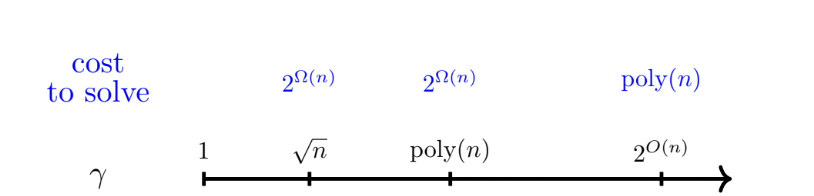
\includegraphics[scale=0.30]{gamma_hard.png}
\end{center}
\end{itemize}
\end{frame}

\subsection{Variantes structurées}
\begin{frame}{Variantes structurées}
\onslide<1->{\textbf{Problème }: LWE tel quel est peu efficace à cause des grandes matrices aléatoires. \\ ~ \\}
\onslide<2->{\textbf{Solution } : Rajouter de la structure : polynômes (Stehlé \textit{et al.} [SSTX09])}
\end{frame}


\begin{frame}{Illustration}
Concrètement, cela consiste à représenter matriciellement le produit de polynômes, et donc à mettre des blocs structurés dans $A$
\begin{center}
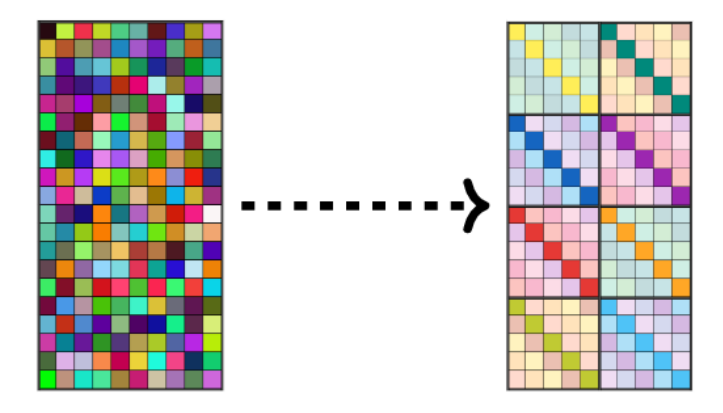
\includegraphics[scale=0.30]{plwe_struct.png}
\end{center}
\end{frame}


\begin{frame}{Variantes structurées}
\onslide<1->{Défaut : nouveau paramètre $f \in \mathbb{Z}^m_p[X]$ qui régit la complexité. \\ ~ \\}
\onslide<1->{\underline{Ex }: $x^n+1$ et $x^n -1$ \\ ~ \\}
\onslide<2->{Roşca \textit{et al.} [RSSS17] introduisent une nouvelle variante structurée, et y réduisent des classes exponentiellement grandes de problèmes P-LWE.}
\end{frame}


\section{Étude de la réduction}


\begin{frame}{Objectif}
\begin{itemize}
\item<1->[•] Comprendre le fonctionnement de la réduction, et son impact sur les paramètres de difficulté.  \\ ~ \\
\item<2->[•] Établir des propriétés sur le nouveau réseau d'arrivée 
\end{itemize}
\end{frame}


\begin{frame}{Représentation matricielle de la réduction}
\onslide<1->{On défini $\text{Rot}_f(a)$ pour qu'elle vérifie $\text{Rot}_f(a) \cdot b = (a\times b \mod f)$ \\ ~ \\}
\onslide<2->{\underline{Ex}: Si $f=x^4+1$ et $\displaystyle a=\sum_{0\leq i < 4} a_ix^i$, alors :
$$
\text{Rot}_f(a) = \begin{pmatrix}
a_0 & a_1 & a_2 & a_3 \\
-a_3 & a_0 & a_1 & a_2 \\
-a_2 & -a_3 & a_0 & a_1 \\
-a_1 & -a_2 & -a_3 & a_0 \\
\end{pmatrix} 
$$
}

\end{frame}

\begin{frame}{Représentation matricielle de la réduction}
\onslide<1->{De même pour $\text{Toep}_d(a)$, choisie pour avoir $\text{Toep}_d(a) \cdot b = (a\odot b)$ \\ ~ \\}
\onslide<2->{\underline{Ex}: Si  $d=3$ et $\displaystyle a=\sum_{0\leq i < 4} a_ix^i$, alors :
$$
\text{Toep}(a) = \begin{pmatrix}
a_0 & a_1 & a_2 & a_3 &0&0&0\\
0&a_0 & a_1 & a_2 & a_3&0&0 \\
0&0&a_0 & a_1 & a_2 & a_3&0 \\
0&0&0&a_0 & a_1 & a_2 & a_3 \\
\end{pmatrix} 
$$
}

\end{frame}


\begin{frame}{Représentation matricielle de la réduction}
La réduction va donc de 
$
\mathcal{L}_1= 
\left[ \begin{array}{c}
\text{Rot}_f(a_1) \\
\vdots  \\
\text{Rot}_f(a_t) \\
\end{array} \right]
$
vers 
$
\mathcal{L}_2= 
\left[ \begin{array}{c}
\text{Toep}_d(a_1) \\
\vdots  \\
\text{Toep}_d(a_t) \\
\end{array} \right]
$

\end{frame}


\section*{Annexe}
\begin{frame}{Références}

\end{frame}
\end{document}













































